\chapter{Målemetode}
\label{ch:measurements}
\fixme{Dette afsnit bør være før realiseringsafsnittet - AB}
Højtalerens frekvenskarakteristik blev målt ved at placere kabinettet i det lyddøde rum. Herved blev eventuelle ekkoer reduceret og den målte frekvenskarakteristik vil derfor ikke blive forstyrret af rummets egen frekvenskarakteristik. Selve karakteristikken blev målt ved hjælp af en såkaldt \textbf{CLIO Pocket}. Dette er et instrument der udsender to 'frekvenschirps' efter hinanden i området fra \SI{10}{\hertz} til \SI{20}{\kilo\hertz}.\fixme{eventuelt kort afsnit, dedikeret til CLIO pocket? - AB}

Ved at måle de de to chirps, så kunne instrumentet måle en forstærkningskurve\fixme{frekvenskarakteristik - AB} i det givne frekvensområde for højtaleren i det pågældende rum. Selve måleopstillingen kan derfor beskrives ved hjælp af blokdiagrammet nedenfor. Det antages at mikrofonens frekvenskarakteristik er ideel i det givne frekvensområde og at luften kun bidrager med en konstant dæmpning ved alle frekvenser. \fixme{Billeder af måleopstillinger - AB}
\begin{figure}[H]
	\centering
	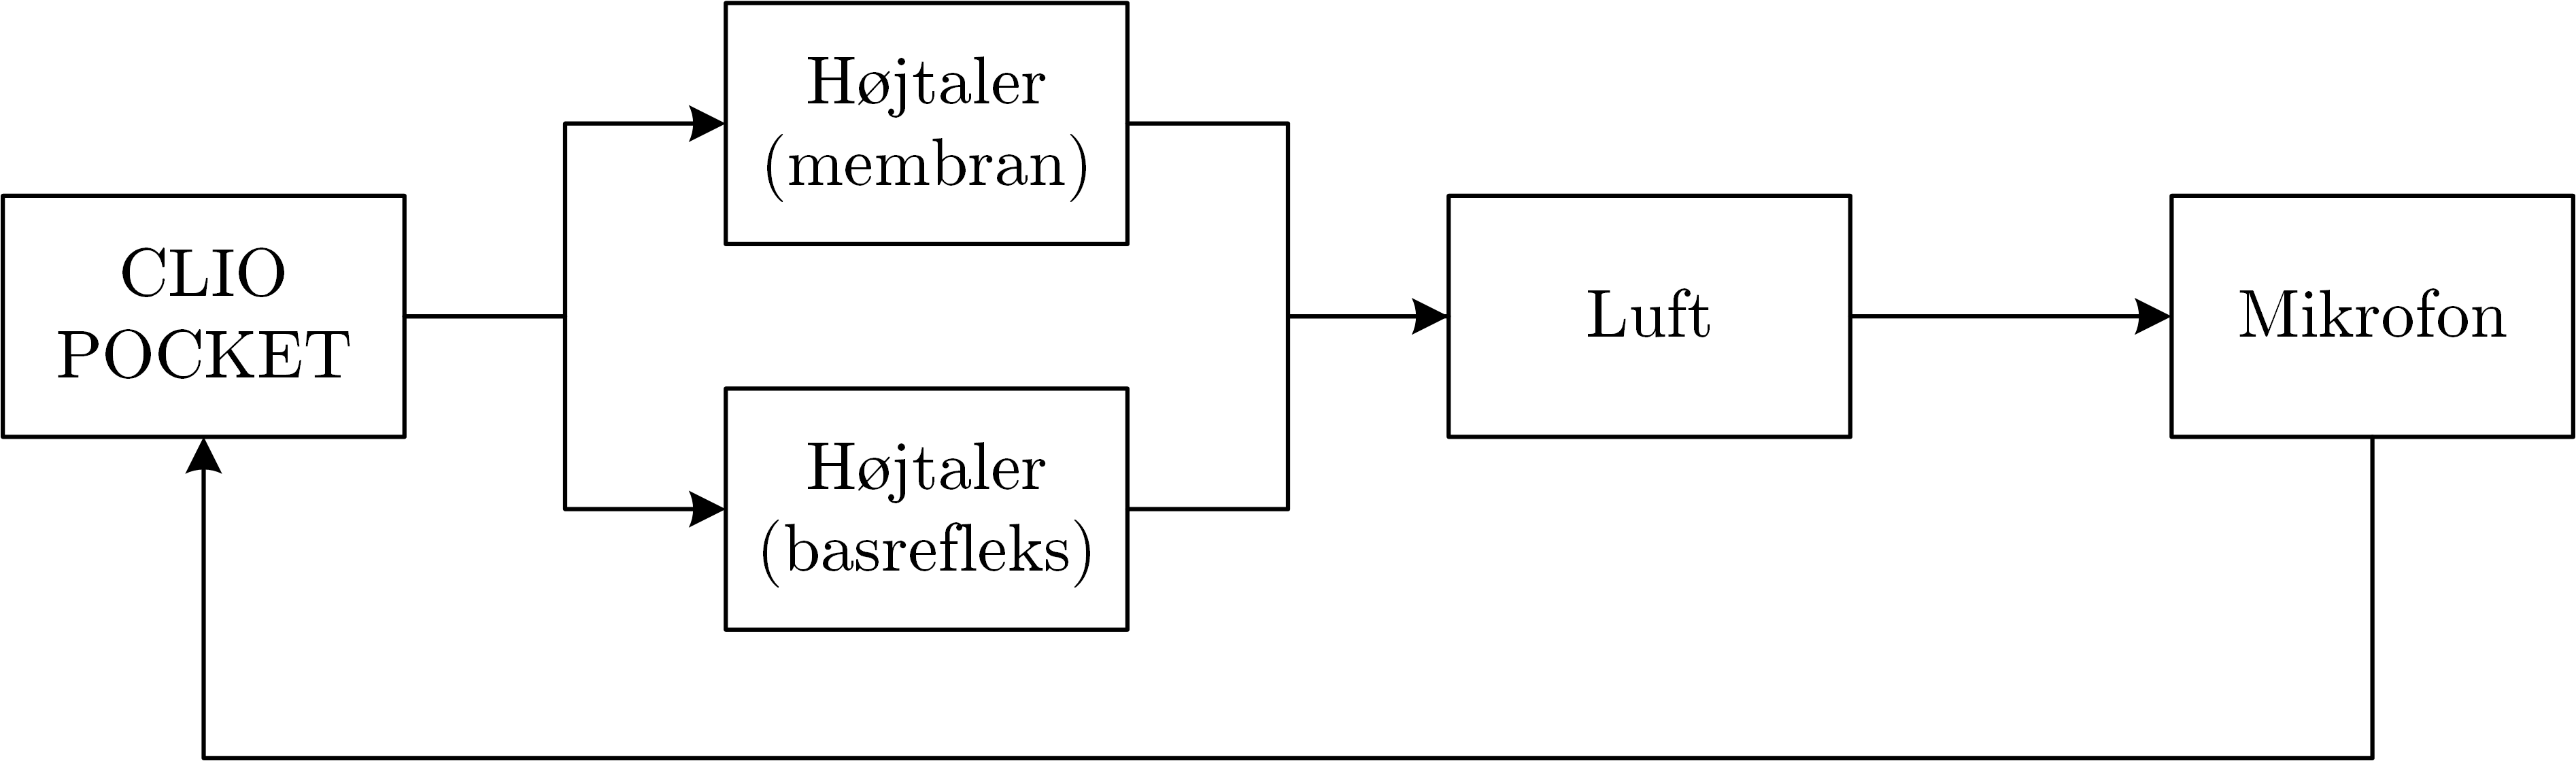
\includegraphics[width=\textwidth]{Pics/CLIOFeedback}
	\caption{CLIO Pocket målemetode}
\end{figure}

Under målingen blev de forskellige størrelser af basrefleksen (lille, mellem og stor) placeret rundt i de udskårne huller i kabinettet (foran, på siden og under) og der blev herefter målt frekvenskarakteristik ved henholdsvis højtalermembranen, basrefleksen og en meter foran højtalerkabinettet (for at simulere hvor en eventuel lytter vil sidde). Derudover blev der også målt på hvordan frekvenskarakteristikken så ud, hvis alle huller var stoppet til - altså et kabinet uden basrefleks. \fixme{Opdelte afsnit mellem referencemålingen i det lyddøde rum og klasselokalet. - AB}